\chapter{Neutrino Identification: Finding MicroBooNE's first Neutrinos} \label{ch:neutrinoID}
The goal of the Neutrino Identification analysis was to positively identify BNB neutrino interactions in the MicroBooNE detector collected during the first days of running. Neutrino event candidates were identified in part by using a cut on detected flash of scintillation light during the 1.6 $\micro s$ beam-spill length of the BNB as well as identifying reconstructed object from the TPC that are neutrino like. After this selection, 2D and 3D event displays were used for verification of the selection performance. This selection was targeted to reduce the ratio of neutrino events to cosmic-only events from the initial 1 neutrino to 675 cosmics to a ratio of 1 to 0.5 or better which is equivalent to a background reduction by a factor of 1000 or more. These selected events were used for MicroBooNE's public displays of neutrino interactions. A clearly visible neutrino interaction with an identifiable vertex and at least 2 tracks originating from the vertex was what the analysis focused on. This analysis wasn't optimized for high purity or efficiency, but rather for very distinguishable neutrino interactions that could be identified by the public.
\section{Flash Finding}
Flash finding is the first step used in finding neutrino interactions. This section will detail how optical information is reconstructed as well as analysis scripts and event filters were used.
\subsection{Flash recinstruction}
A flash is described as a collection of light seen at the same time within the detector. They are then reconstructed by identifying signal from the PMTs above a specific photoelectron (PE) threshold. These signals are called optical hits. Optical hits from all the PMTs are then accumulated into 1 $\micro s$ bins of time. If a specific bin is above a set PE threshold, then the optical hits that overlap in time are the labeled as the hits from the flash. All flash reconstructed properties like average time and x/y positions are then found via the flash labeled optical hits. The total size of the flash is found by summing up the total number of photoelectrons from all PMTs. Neutrino interactions and cosmic muons will have a larger flash size compared to noise and other low-energy backgrounds, therefore a total PE cut is used to reject these backgrounds. A total PE cut of 50 PE was deemed sufficient for this analysis. Figures \ref{fig:totalpe} and \ref{fig:totalpe_zoomed} show the total PE versus the selection efficency of selecting neutrino beam events. 


\begin{figure}[htp!]
\centering
	\begin{subfigure}[b]{.4\textwidth}
	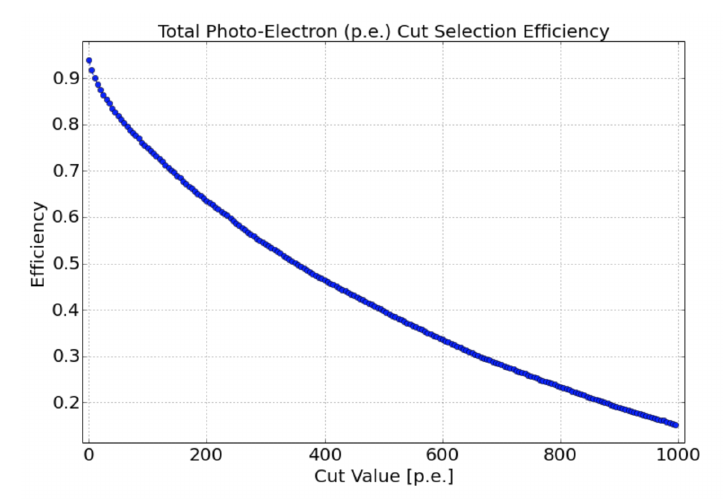
\includegraphics[width=\textwidth]{figs/totalpecut.png}
	\caption{Efficiency for selecting beam events as a function of minimum total PE cut.}
	\label{fig:totalpe}
	\end{subfigure}
	\quad
	\begin{subfigure}[b]{.4\textwidth}
	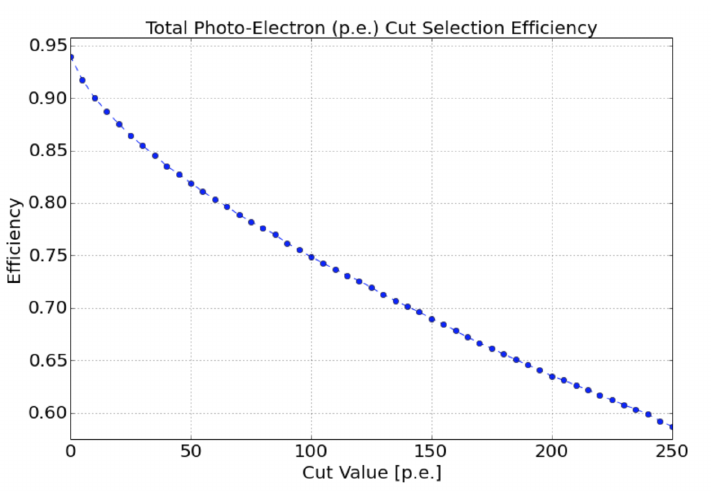
\includegraphics[width=\textwidth]{figs/totalpe_zoomed.png}
	\caption{Efficiency for selecting beam events as a function of minimum total PE cut. Zoomed into interesting region.}
	\label{fig:totalpe_zoomed}
	\end{subfigure}
	\quad
\label{fig:PE}
\end{figure}
